\chapter{Hintergrund und Stand der Technik}

\section{Network-On-Chip (NoC)}
Ein Network-on-Chip ist ein Kommunikationssystem, das in modernen System-on-Chip (SoC) Architekturen verwendet wird, um verschiedene Komponenten (z.B. Prozessoren, Speicher und spezialisierte Einheiten) effizient miteinander zu verbinden. Statt klassische Busse oder Punkt-zu-Punkt-Verbindungen zu nutzen, setzt NoC auf ein netzwerkartiges Kommunikationsprinzip, das von Computernetzwerken oder Hochleistungsrechnern inspiriert ist. \TODO{Add References}

Die Grafik~\ref{fig:Evolution_of_Interconnection} zeigt die Entwicklung der Bus-Technologien der vergangenen Jahre.
\begin{figure}[htbp]
    \centering
    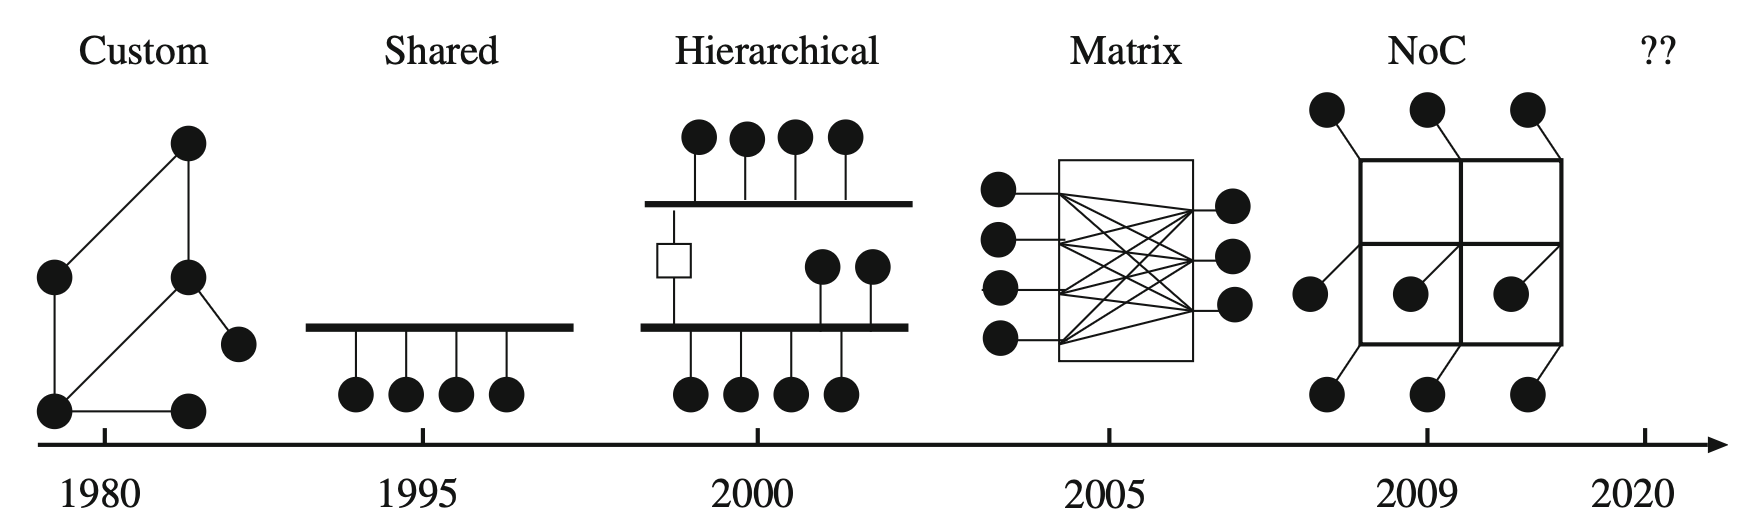
\includegraphics[width=0.95\textwidth]{img/Evolution of On-Chip communication interconnect.png}
    \caption{Evolution of Interconnections}~\cite{BenAbdallah2013}  \label{fig:Evolution_of_Interconnection}
\end{figure}

Vor 1980 wurden in der Regel maßgeschneiderte (Custom) Lösungen für die On-Chip-Kommunikation verwendet. Ab etwa 1995 kamen sogenannte Shared-Bus-Architekturen wie ARM's AMBA-Bus\TODO{ar} und IBM's CoreConnect\TODO{ar} zum Einsatz. Diese Ansätze ermöglichten ein modulareres Design mit standardisierten Schnittstellen und unterstützten die Wiederverwendung von IP-Komponenten (IP-Reuse).
Mit zunehmendem Bandbreitenbedarf stellten sich Shared-Bus-Systeme jedoch als Engpass (Bottleneck) heraus. Um dieses Problem zu umgehen, wurden hierarchische Busarchitekturen eingeführt. Diese nutzen mehrere Busse oder Bussegmente, um die Last des Hauptbusses zu verringern. Lokale Kommunikation zwischen Modulen auf demselben Bussegment ist so möglich, ohne den gesamten Bus zu belasten. Allerdings sind solche Architekturen nur begrenzt skalierbar, wenig flexibel und führen zu steigender Designkomplexität. Je mehr Kerne angeschlossen sind, desto schwieriger wird es, Timing-Vorgaben (Time Closure) und Quality-of-Service (QoS) sicherzustellen.\TODO{Begrifflichkeiten erläutern}
Eine weitere Alternative stellte die Bus-Matrix dar – ein vollständiges Crossbar-System, das parallele Verbindungen zwischen Komponenten erlaubt. Doch auch hier steigt mit zunehmender Systemgröße die Komplexität der Verdrahtung und kann schließlich den Aufwand für die Logik selbst übersteigen. Zudem trennen solche Systeme nicht klar zwischen Transport-, Transaktions- und physikalischer Schicht. Wird also ein Systemupgrade erforderlich, betrifft dies häufig das gesamte Schnittstellendesign sowie alle daran angeschlossenen Blöcke.
Vor diesem Hintergrund schlugen einige Forscher Anfang der 2000er Jahre vor, die Kommunikation zwischen verschiedenen Recheneinheiten auf einem Chip über eine vordefinierte Plattform zu realisieren – ein integriertes Schaltnetzwerk, bekannt als Network-on-Chip (NoC). NoCs erfüllen zentrale Anforderungen moderner SoCs: Wiederverwendbarkeit, skalierbare Bandbreite sowie Energieeffizienz. NoC haben die verdrahteten Verbindungen ersetzt und nutzen dafür intelligente Netzwerkinfrastrukturen. Hierbei bedient sich NoC an Modellen, Techniken und Werkzeugen der Netzwerkkommunikation, sodass festverdrahtete Kommunikation durch Paketübertragung ersetzt wird.\TODO{ar}

Ein NoC besteht aus den folgenden drei wesentlichen Komponenten:
\begin{enumerate}
    \item \textbf{Links}, die physisch die Knoten (Nodes) miteinander verbinden und die Kommunikation zwischen ihnen ermöglichen. Ein Link verbindet jeweils zwei Router (siehe Punkt 2). Ein Link kann einen oder mehrere logische Kanäle enthalten; ein Kanal wiederum besteht aus einem Satz von Leitungen (Kabeln). Die Implementierung eines Links umfasst auch die Definition des Synchronisierungsprotokolls zwischen dem Quell- und dem Zielknoten.
    \item \textbf{Router}, die für die Umsetzung des Kommunikationsprotokolls verantwortlich sind. Ein Router verfügt über mehrere Eingangs- und Ausgangsports sowie über eine Switching-Matrix, die die Verbindung zwischen diesen Ports herstellt. Zusätzlich besitzt jeder Router einen lokalen Port, der mit dem jeweiligen IP-Kern verbunden ist. Ein Logikblock innerhalb des Routers steuert die Flusskontrolle (Flow Control Policies) und legt die allgemeine Strategie für die Datenweiterleitung fest.\TODO{Flusskontrolle erklären}
    \item \textbf{Network Adapter (NA)} bzw. \textbf{Network Interface (NI)} stellen die logische Schnittstelle zwischen den IP-Kernen (IP Cores) und dem Netzwerk (NoC) dar. Sie sind notwendig, da die internen Kommunikationsmechanismen eines IP-Kerns (z.B. Busprotokolle wie AXI) typischerweise nicht direkt mit den paketbasierten Mechanismen eines NoC kompatibel sind.
\end{enumerate}

Network-on-Chip (NoC) können durch die Struktur ihrer Router-Verbindungen charakterisiert werden. Diese Struktur wird auch als \textit{Topologie} bezeichnet und typischerweise als Graph $G(N, C)$ dargestellt, wobei $N$ die Menge der Router (Nodes) und $C$ die Menge der Kanäle (Edges) repräsentiert. Man unterscheidet dabei grundsätzlich zwischen \textit{direkter} und \textit{indirekter Topologie}.
Bei der \textit{direkten Topologie} ist jedem Router genau ein Prozessor zugeordnet. Dieses Paar wird als Knoten (Node) im Netzwerk betrachtet. Jede Node ist mit einer festen Anzahl von Nachbarn verbunden, und Nachrichten werden über eine oder mehrere Zwischenknoten (Router) transportiert. Häufig verwendete Strukturen sind dabei n-dimensionale Gitter (grids), Mesh-Topologien oder Torus-Topologien (auch k-ary n-cubes genannt).
In der \textit{indirekten Topologie} sind nicht alle Router direkt mit einer Processing Unit verbunden, wie es beim direkten Modell der Fall ist. Einige Router dienen ausschließlich dazu, Nachrichten durch das Netzwerk zu routen, während andere für Steuerungs- und Verwaltungsfunktionen zuständig sind. Diese sogenannten Logikrouter fungieren dabei als Quelle (Source) oder Ziel (Target) von Nachrichten.

In NoC-Architekturen stellt das Routing einen zentralen Bestandteil dar, da es darüber entscheidet, wie Datenpakete zwischen den einzelnen Knotenpunkten übertragen werden. Grundsätzlich lassen sich Routing-Algorithmen in zwei Hauptkategorien einteilen: Deterministisches und adaptives Routing. Beim \textit{deterministischen Routing} ist der Pfad, den ein Paket von der Quelle zum Ziel nimmt, im Voraus festgelegt und bleibt unabhängig von der aktuellen Netzwerkauslastung oder anderen Rahmenbedingungen unverändert. Zu den bekanntesten deterministischen Verfahren zählen das XY-Routing sowie das Dimension-Order-Routing (DOR). Im Gegensatz dazu ermöglicht \textit{adaptives Routing} eine dynamische Pfadanpassung basierend auf dem aktuellen Zustand des Netzwerks. Dadurch können beispielsweise Engpässe oder fehlerhafte Verbindungen umgangen werden. Zu den adaptiven Algorithmen zählen unter anderem DyAD (Dynamic Adaptive Deterministic) sowie das Odd-Even-Routing.

Ergänzend existieren \textit{staukontrollierte Routing-Algorithmen}, die gezielt die aktuelle Auslastung des Netzwerks berücksichtigen, um eine möglichst gleichmäßige Verteilung des Datenverkehrs zu erreichen. Eine besondere Unterkategorie stellen sogenannte \textit{ant-kolonie-basierte Algorithmen} dar, welche Konzepte der Schwarmintelligenz nutzen. Hierbei werden Pfade mithilfe von virtuellen Pheromonspuren erlernt und laufend optimiert, was eine flexible und anpassungsfähige Routenfindung ermöglicht.

Ein weiterer wesentlicher Aspekt in NoC-Systemen ist die sogenannte Flow Control, die festlegt, wie verfügbare Ressourcen wie Bandbreite oder Pufferspeicher den einzelnen Datenpaketen zugewiesen werden. Ziel ist es, eine möglichst effiziente Ressourcennutzung zu gewährleisten und dadurch den Gesamtdurchsatz des Netzwerks zu optimieren. Grundsätzlich unterscheidet man zwischen bufferloser und gepufferter Flusskontrolle. Bei \textit{bufferloser Flow Control} existieren keine oder nur sehr begrenzte Zwischenspeicher; Datenpakete, die nicht sofort weitergeleitet werden können, werden entweder verworfen oder über alternative Routen umgeleitet. Ein typisches Beispiel hierfür ist das Circuit Switching, bei dem vor der Datenübertragung ein fester Pfad durch das Netzwerk reserviert wird. Bei der gepufferten Flow Control hingegen werden Datenpakete vorübergehend zwischengespeichert, wenn der gewünschte Ausgangskanal belegt ist oder das Weiterleiten anderweitig verzögert wird. Diese Methode erhöht die Flexibilität der Datenübertragung und reduziert die Wahrscheinlichkeit von Paketverlusten oder Umleitungen, geht jedoch mit einem höheren Hardwareaufwand und Energieverbrauch einher, da zusätzliche Pufferressourcen bereitgestellt und verwaltet werden müssen.

Innerhalb der \textit{gepufferten Flusskontrolle} lassen sich zwei zentrale Ansätze unterscheiden: Beim Packet-Buffer Flow Control wird das gesamte Paket in einem Puffer gespeichert, bis es vollständig weitergeleitet werden kann. Diese Methode ist einfach zu implementieren, kann jedoch ineffizient sein, insbesondere bei großen Paketen und begrenztem Pufferspeicher. Eine feinere Kontrolle bietet die Flit-Buffer Flow Control, bei der Pakete in kleinere Einheiten, sogenannte Flits (Flow Control Digits), aufgeteilt und einzeln gepuffert werden. Dadurch kann der verfügbare Speicher effizienter genutzt und der Datenfluss besser koordiniert werden, was zu einer höheren Netzwerkleistung führen kann.

Zusätzlich existieren verschiedene Pufferstrategien innerhalb dieser Ansätze, darunter \textit{Input Buffering}, \textit{Output Buffering} sowie \textit{Virtual Channel Buffering}. Beim Input Buffering werden eingehende Datenflüsse an jedem Eingangskanal zwischengespeichert, während beim Output Buffering die Puffer an den Ausgangskanälen eines Routers positioniert sind. Virtual Channel Buffering wiederum erlaubt mehreren logischen Kanälen, sich einen physischen Kanal zu teilen, wodurch Blockierungen reduziert und die Ausnutzung der verfügbaren Bandbreite verbessert werden können. Diese Technik erfordert jedoch eine komplexere Steuerlogik und erhöht den Hardwareaufwand.

Kangmin hat in seinem Artikel von 2006 ein NoC-Protokoll-Design vorgestellt:
\begin{figure}[htbp]
    \centering
    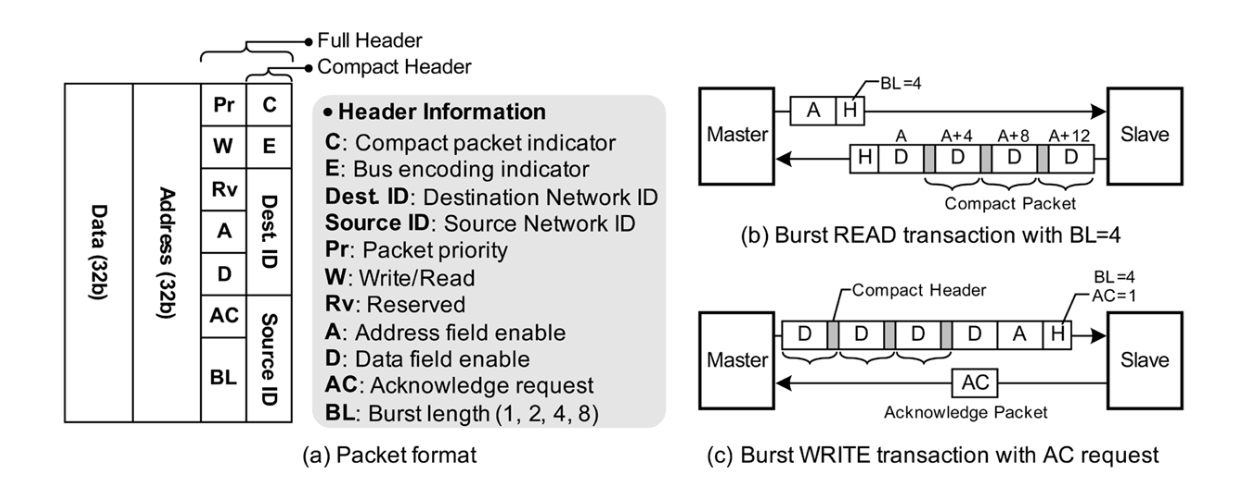
\includegraphics[width=0.95\textwidth]{img/NoC Protocol.png}
    \caption{NoC-Protokol~\cite{kangmin_low-power_2006}}\label{fig:NOC_Protocol}
\end{figure}

\TODO{Vor- und Nachteile}


\section{AXI4-Protokoll}

\section{QoS-Konzepte}

\section{Vergleichbare Literaturansätze}
